\documentclass[12pt]{amsart}
\usepackage[english]{babel}
\usepackage[left=0.75in, right=0.75in, bottom=0.75in, top=0.75in]{geometry}
\usepackage[utf8x]{inputenc}
\usepackage{amsmath,amssymb,amsthm}
\usepackage{enumerate}
\usepackage{graphicx}

\usepackage[table,dvipsnames]{xcolor}
\usepackage{pgf,tikz,tikz-3dplot}
\usetikzlibrary{shapes,arrows,positioning,backgrounds}
\tikzset{%
	goodnode/.style={circle, draw=MidnightBlue!90, thick, fill=gray!40},
	okaynode/.style={circle, draw=Orange!90, thick, fill=gray!40},
	badnode/.style={circle, draw=Red!90, thick, fill=gray!40},
	togood/.style={draw=MidnightBlue, thick,->,>=stealth',shorten >=1pt},
	tookay/.style={draw=Orange, thick,->,>=stealth',shorten >=1pt},
	tobad/.style={draw=Red, thick,->,>=stealth',shorten >=1pt}}

\usepackage{float}

\title{OPER 640 - Stochastic Modeling and Analysis}
\author{B. Hosley}
\date{\today}

\begin{document}
	\maketitle
	\raggedbottom

\section{Description}

% Problem description
% 	Paraphrase project description,
% 	formulate analysis questions of interest to leadership

\section{Modeling the Situation}

%DTMC model formulation (Lesson2 slide 18 (with single entity transition diagram))

% Define Xn as the state of the system at time n or the n-th observation (or event)
% Define the state space S as the set of all possible outcomes for Xn
% Verify the Markov Property is satisfied.
% Verify Time-Homogeneity
% Construct the Transition Probability Matrix. Or specify probability function p_ij.
% As needed:
% 	Formulate state transition function (X_n+1 as a function of X_n)
% 	Draw a Transition Diagram.
% 	Define a cost or reward function.

Figure \ref{DTMC} shows the life-cycle of an individual aircraft.

\begin{figure}[H]
	\centering
	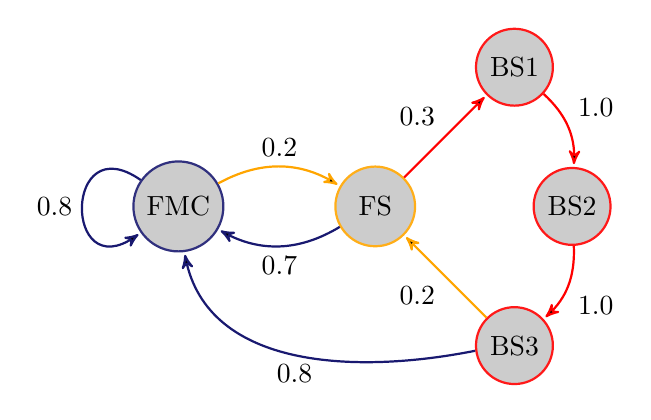
\begin{tikzpicture}[node distance=2.5cm]		
		\node[goodnode] (FMC) {FMC};
		\node[okaynode] (FS) [right of=FMC] {\(\ \)FS\(\ \)};
		\node[badnode] (BS1) [above right of=FS] {BS1};
		\node[badnode] (BS2) [right of=FS] {BS2};
		\node[badnode] (BS3) [below right of=FS] {BS3};
		
		\path[togood] (FMC) 	edge [loop left, min distance=12mm, out=145, in=215]  node [left] 	{\(0.8\)} (FMC);
		\path[togood] (FS)  	edge [bend left]  node [below] 	{\(0.7\)} (FMC);
		\path[togood] (BS3) 	edge [bend left, in=120]  node [below] 	{\(0.8\)} (FMC);
		
		\path[tookay] (FMC) 	edge [bend left]  node [above] 	{\(0.2\)} (FS);
		\path[tookay] (BS3) 	edge []  node [below left] 	{\(0.2\)} (FS);
		
		\path[tobad]  (FS) 		edge []  node [above left] 	{\(0.3\)} (BS1);
		\path[tobad]  (BS1) 	edge [bend left=25]  node [above right] 	{\(1.0\)} (BS2);
		\path[tobad]  (BS2) 	edge [bend left=25]  node [below right] 	{\(1.0\)} (BS3);
	\end{tikzpicture}
	\caption{Single Entity DTMC.}
	\label{DTMC}
\end{figure}



\section{Baseline Analysis}

% Baseline analysis - primary analysis questions
% 	How often will the squadron be able to achieve mission success, meeting 8-orbit mission requirements
% 	How long will it take for the squadron become FMC >= 8 aircraft
% 	What is the long-term sortie generation rate?
% 	What is the long-term mission capable aircraft availability rate?

\section{Exploratory Analysis}

% Sensitivity (excursion) analyses - the what-if questions, 
% 	explore possible solutions by modifying parameter values

\section{Conclusions and Recommendations}

% Conclusions and recommendations


\end{document}